\subsection{Cyclic dependencies}
A cyclic dependency, as depicted in \cref{tikz:cyclic}, arises when a set of packages depend on each other making it impossible to import them independently. Cyclic dependencies are considered bad practice in software engineering because they introduce a tight coupling between the packages making them difficult to re-use or modify~\cite{whats_wrong_with_circular_references}.

\begin{figure}[tb]
\begin{center}
\setfigname{}\begin{tikzpicture}[->,>=stealth',shorten >=1pt,auto,node distance=3cm,
  thick,main node/.style={circle,fill=blue!20,draw,font=\sffamily\Large\bfseries}]

  \node[main node] (b) {B};
  \node[main node] (a) [below left of=b] {A};
  \node[main node] (c) [below right of=b] {C};

  \path[every node/.style={font=\sffamily\small}]
    (b) edge node [left] {} (c)
    (c) edge node [right] {} (a)
    (a) edge node [right] {} (b);
\end{tikzpicture}
\end{center}
\caption{An example depicting three packages A, B and C with a cyclic relationship. A imports B, B imports C and C imports A.}
\label{tikz:cyclic}
\end{figure}

A structural analysis of PIPE 4 was performed by the Stan4J standalone tool. It reports cyclic dependencies as tangles and considers a tangle to be `A subgraph with at least two nodes, where each node is reachable from each other. Every cycle lies in a tangle and every tangle consists of just cycles'~\cite{stan_whitepaper}. It reports PIPE 4 as 29.17\% tangled which can be seen diagrammatically in~\cref{fig:tangle}.

\begin{figure}[p]
\begin{center}
    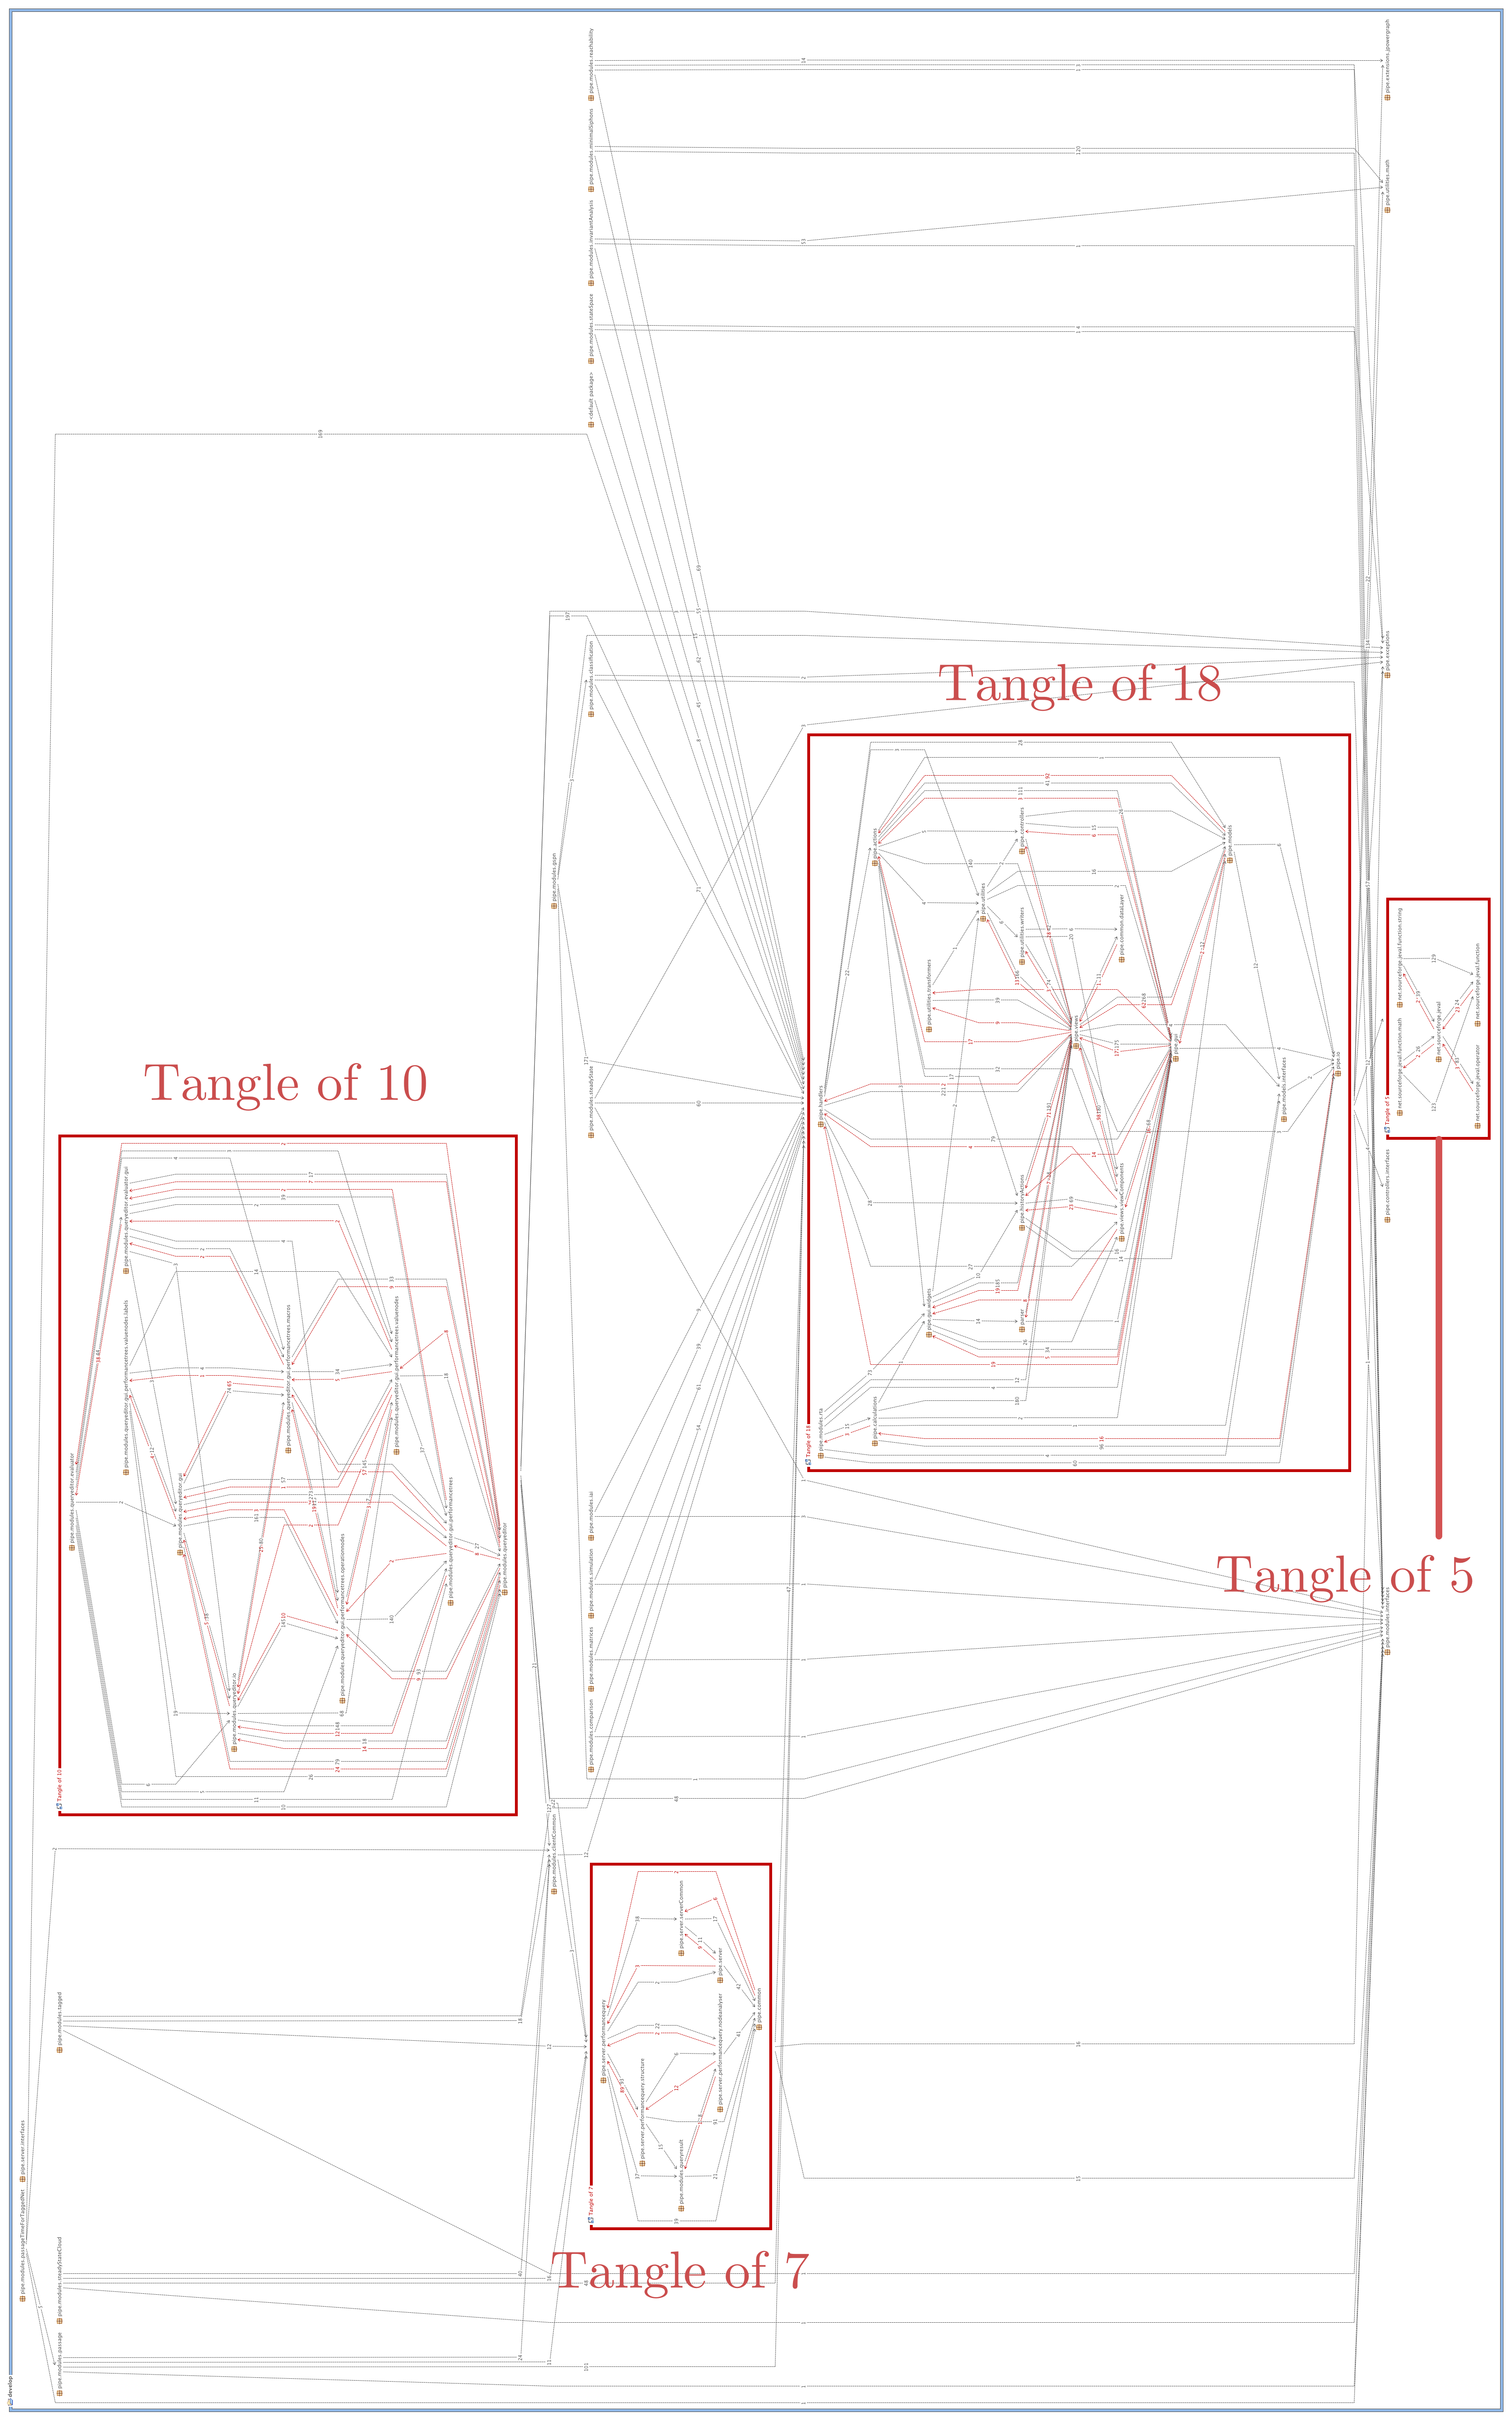
\includegraphics[width=0.8\textwidth]{analysis/tangle_annotated.png} 
    \caption{Stan4J tangle graph of the entire pre-existing PIPE codebase. It has 4 distinct tangles which are of sizes 18, 10, 7 and 5.}
    \label{fig:tangle}
\end{center}
\end{figure}

% \input{pipe_architecture/standards/tikz/tangle}

Ideally PIPE should have as few tangles as possible.